%%%%%%%%%%%%%%%%%%%%%%%%%%%%%%%%%%%%%%%%%
% Beamer Presentation
% LaTeX Template
% Version 1.0 (10/11/12)
%
% This template has been downloaded from:
% http://www.LaTeXTemplates.com
%
% License:
% CC BY-NC-SA 3.0 (http://creativecommons.org/licenses/by-nc-sa/3.0/)
%
%%%%%%%%%%%%%%%%%%%%%%%%%%%%%%%%%%%%%%%%%

%----------------------------------------------------------------------------------------
%	PACKAGES AND THEMES
%----------------------------------------------------------------------------------------

\documentclass{beamer}

\mode<presentation> {

% The Beamer class comes with a number of default slide themes
% which change the colors and layouts of slides. Below this is a list
% of all the themes, uncomment each in turn to see what they look like.

%\usetheme{default}
%\usetheme{AnnArbor}
%\usetheme{Antibes}
%\usetheme{Bergen}
%\usetheme{Berkeley}
%\usetheme{Berlin}
%\usetheme{Boadilla}
\usetheme{CambridgeUS}
%\usetheme{Copenhagen}
%\usetheme{Darmstadt}
%\usetheme{Dresden}
%\usetheme{Frankfurt}
%\usetheme{Goettingen}
%\usetheme{Hannover}
%\usetheme{Ilmenau}
%\usetheme{JuanLesPins}
%\usetheme{Luebeck}
%\usetheme{Madrid}
%\usetheme{Malmoe}
%\usetheme{Marburg}
%\usetheme{Montpellier}
%\usetheme{PaloAlto}
%\usetheme{Pittsburgh}
%\usetheme{Rochester}
%\usetheme{Singapore}
%\usetheme{Szeged}
%\usetheme{Warsaw}
% As well as themes, the Beamer class has a number of color themes
% for any slide theme. Uncomment each of these in turn to see how it
% changes the colors of your current slide theme.

%\usecolortheme{albatross}
\usecolortheme{beaver}
%\usecolortheme{beetle}
%\usecolortheme{crane}
%\usecolortheme{dolphin}
%\usecolortheme{dove}
%\usecolortheme{fly}
%\usecolortheme{lily}
%\usecolortheme{orchid}
%\usecolortheme{rose}
%\usecolortheme{seagull}
%\usecolortheme{seahorse}
%\usecolortheme{whale}
%\usecolortheme{wolverine}

%\setbeamertemplate{footline} % To remove the footer line in all slides uncomment this line
\setbeamertemplate{footline}[page number] % To replace the footer line in all slides with a simple slide count uncomment this line

%\setbeamertemplate{navigation symbols}{} % To remove the navigation symbols from the bottom of all slides uncomment this line
}
\usepackage{bbm}
\usepackage{tikz}
\usetikzlibrary{graphs}
\usetikzlibrary{overlay-beamer-styles}
\newcommand{\tikzmark}[1]{\tikz[remember picture] \node[coordinate] (#1) {#1};}
\usepackage{verbatim}
\usetikzlibrary{arrows,shapes}
\usepackage{graphicx} % Allows including images
\usepackage{mathtools}
%\usepackage{amsmath}
\newcommand\scalemath[2]{\scalebox{#1}{\mbox{\ensuremath{\displaystyle #2}}}}
\newcommand\numberthis{\addtocounter{equation}{1}\tag{\theequation}}
\usepackage{booktabs} % Allows the use of \toprule, \midrule and \bottomrule in tables
\usepackage{hyperref}
\usepackage[font=footnotesize,justification=centering]{caption}
\tikzset{
  invisible/.style={opacity=0},
  visible on/.style={alt={#1{}{invisible}}},
  alt/.code args={<#1>#2#3}{%
    \alt<#1>{\pgfkeysalso{#2}}{\pgfkeysalso{#3}} % \pgfkeysalso doesn't change the path
  },
  marked/.style={
    %color=white,
    fill=green!20,
  },
  marked on/.style={alt=#1{marked}{}}
  }
  \setbeamercovered{transparent}
%\usepackage{algorithm,algorithmic}
\usepackage[font=footnotesize,justification=centering]{caption}
\usepackage[ruled,vlined,linesnumbered]{algorithm2e}
\usepackage{caption}
\usepackage{booktabs}
\usepackage{array}
\usepackage{multirow}
\usepackage{balance}
\usepackage{slashbox}
\usepackage{hhline}
%----------------------------------------------------------------------------------------
%	TITLE PAGE
%----------------------------------------------------------------------------------------

\title[ADMM FPGA]{An Embedded Scalable Linear Model Predictive Hardware-based Controller using ADMM} % The short title appears at the bottom of every slide, the full title is only on the title page

\author{Pei Zhang, Joseph Zambreno and Phillip H. Jones} % Your name
\institute[ISU] % Your institution as it will appear on the bottom of every slide, may be shorthand to save space
{
\textit{Presenter: Pei Zhang}\\
\medskip
Iowa State University\\ % Your institution for the title page
\medskip

\textit{peizhang@iastate.edu} % Your email address
}
\date{\today} % Date, can be changed to a custom date



\begin{document}


\begin{frame}
\titlepage % Print the title page as the first slide
\end{frame}

\begin{frame}
\frametitle{Overview} % Table of contents slide, comment this block out to remove it
\tableofcontents % Throughout your presentation, if you choose to use \section{} and \subsection{} commands, these will automatically be printed on this slide as an overview of your presentation
\end{frame}

%----------------------------------------------------------------------------------------
%	PRESENTATION SLIDES
%----------------------------------------------------------------------------------------

\section{Related Work}
%------------------------------------------------
\begin{frame}
\frametitle{Quadratic Programming (QP) solutions}

MPC can be posed as a Quadratic Programming problem.\\~\\

QP problems can be solved reliably via various iterative methods.
\begin{itemize}
\item Interior-Point Method (IPM)
\item Active Set Method (ASM)
\item Splitting Method
\end{itemize}

\end{frame}
%------------------------------------------------

%------------------------------------------------
\begin{frame}
\frametitle{FPGA-based QP solutions}
Compare IPM and ASM in FPGA\\~\\
\begin{itemize}
\item ASM gives lower computing complexity and converges faster when the number of decision variables and constraints are small.
\item IPM is a better choice when considering scalability.
\end{itemize}
\end{frame}
%------------------------------------------------


\section{Background}
\subsection{State Space Model}
%------------------------------------------------
\begin{frame}
\frametitle{State Space Model}
A discrete state-space model defines what state a system will be in one-time step into the future:
\begin{equation}
\label{eq:xk}
x_{k+1}=A x_k + B u_k 
\end{equation}  
\begin{equation}
\label{eq:yk}
y_{k}=C x_k + D u_k  
\end{equation}  
\begin{itemize}
  \item $x_k$ represents the state of the system at time $k$
  \item $u_k$ represents the input acting on the system at time $k$
  \item $y_k$ represents outputs of the system at time $k$
  \item $A$ is a matrix that defines the internal dynamics of the system
  \item $B$ is a matrix that defines how the input acting upon the system impact its state
  \item $C$ is a matrix that transforms states of the system into outputs ($y_k$)
\end{itemize}
\end{frame}
%------------------------------------------------


\subsection{Model Predictive Optimal Control}
%------------------------------------------------

\begin{frame}
\frametitle{Augmented Vector}
\begin{equation}
\scalemath{0.8}{
U_k=
\begin{bmatrix}
u_k\\
u_{k+1}\\
\vdots \\
u_{k+H_u}
\end{bmatrix}
\text{,}\quad
\Delta U_k=
\begin{bmatrix}
\Delta u_k\\
\Delta u_{k+1}\\
\vdots \\
\Delta u_{k+H_{u-1}}
\end{bmatrix}
\text{,}\quad
X_k=
\begin{bmatrix}
x_k\\
x_{k+1}\\
\vdots \\
x_{k+H_p}
\end{bmatrix}\label{eq:aug}}
\end{equation}
Where:
\begin{itemize}
	\item $H_u$: changeable future input horizon. We assume input $u_k$ will be constant after $H_u$ time steps.
	\item $H_p$: prediction horizon. Normally, $H_p\geq H_u$. 
	\item $U_k \in \mathbb{R}^{M(H_{u}+1)}$, $\Delta U_k \in \mathbb{R}^{MH_{u}}$, $X_k \in \mathbb{R}^{N(H_{p}+1)}$.
\end{itemize}
\end{frame}
%------------------------------------------------
%------------------------------------------------
\begin{frame}
\frametitle{Cost Function}
Cost function:
\begin{equation}
\scalemath{0.8}{
\begin{split}
\mathbb{C}(k)=\frac{1}{2}\Big( \sum_{i=k}^{k+H_p}(x_i^Tq_ix_i-2r_i^Tq_ix_i)+\sum_{i=k}^{k+H_u}u_i^Tp_iu_i+\sum_{i=k}^{k+H_{u-1}}\Delta u_i^Ts_i\Delta u_i\Big)+Const
\label{eq:costf}
\end{split}}
\end{equation}

Compact matrix format:
\begin{equation}
\scalemath{0.8}{
\mathbb{C}(k)=\frac{1}{2}
\begin{bmatrix}
X_k\\
U_k\\
\Delta U_k
\end{bmatrix}^T
\begin{bmatrix}
Q& & \\
 &P& \\
& &S 
\end{bmatrix}
\begin{bmatrix}
X_k\\
U_k\\
\Delta U_k
\end{bmatrix}
-
R_k^TQX_k}
\end{equation}
\end{frame}
%------------------------------------------------
%------------------------------------------------
\begin{frame}
\frametitle{Box Constraints}
\framesubtitle{Constraints in the QP Problem}
The state $X_k$, input $U_k$ and input rate of change $\Delta U_k$ are constrained by its lower and upper value respectively:
\[
  \begin{cases*}
    min(x) \leq x_k \leq max(x)\\
    min(\Delta u) \leq \Delta u_k \leq max(\Delta u)\\
    min(u) \leq u_k \leq max(u)
  \end{cases*}\]
\end{frame}
%------------------------------------------------


\subsection{Splitting Method}
%------------------------------------------------


\begin{frame}  
\frametitle{Consensus Form}
One technique for partitioning variables in ADMM is writing the convex QP problem into consensus form:

\begin{align*}
&minimize:\;  \tikz[baseline,remember picture]{\node[anchor=base,marked on=<2->] (t1){$\mathbbm{1}_{\mathcal{D}}(\chi)+\phi(\chi)$};} + \tikz[baseline,remember picture]{\node[anchor=base,marked on=<2->] (t2){$\mathbbm{1}_{\mathcal{C}}(\zeta)$};}\\
&subject\;  to:\; \chi=\zeta
\end{align*}

\hspace{35.3 mm} \visible<2->{\tikz[baseline,remember picture]{\node[fill=green!20,anchor=base] (n1){$g(\chi)$};}}
\hspace{15.3 mm} \visible<2->{\tikz[baseline,remember picture]{\node[fill=green!20,anchor=base] (n2){$f(\zeta)$};}}
%\tikz[remember picture] \node[coordinate] (n1) {};

\begin{tikzpicture}[remember picture,overlay]   %% use here too
        \path[draw=magenta,thick,->]<2->([yshift=0mm,xshift=0mm]n1.north) to [out=0, in=0,distance=-0.1in] (t1.south);
\end{tikzpicture}

%\tikz[remember picture] \node[coordinate] (n2) {};
\begin{tikzpicture}[remember picture,overlay]   %% use here too
        \path[draw=magenta,thick,->]<2->([yshift=0mm,xshift=0mm]n2.north) to [out=0, in=0in,distance=-0.1in] (t2.south);
\end{tikzpicture}

%\begin{align*}
%&minimize:\;  \mathbbm{1}_{\mathcal{D}}(\chi)+\phi(\chi) +\mathbbm{1}_{\mathcal{C}}(\zeta)\\
%&subject\;  to:\; \chi=\zeta
%\end{align*}

\end{frame}
%------------------------------------------------

%------------------------------------------------
\begin{frame}  
\frametitle{Consensus Form}
\begin{align*}
&g(\chi)=\mathbbm{1}_{\mathcal{D}}(\chi)+\phi(\chi)\\
&f(\zeta)=\mathbbm{1}_{\mathcal{C}}(\zeta) 
\numberthis \label{eq:gf}
\end{align*}
\begin{align}
&\chi^{i+1}:=prox_{g,\rho}(\zeta^i+\upsilon^i)\label{eq:xi}\\
&\zeta^{i+1}:=prox_{f,\rho}(\chi^{i+1}+\upsilon^i)\label{eq:zi}\\
&\upsilon^{i+1}:=\upsilon^i+\rho (\chi^{i+1}-\zeta^{i+1})\label{eq:vi}
\end{align}
Here, $i$ is the iteration counter, $prox_{f,\rho}(\chi)$ is the proximal mapping (or proximal operator) of a convex function $f$: 
\begin{equation*}
prox_{f,\rho}(\chi)=arg\;\underset{u}{\min}(f(u)+\frac{\rho}{2}\| \chi-u\| _2^2)
\end{equation*}
$\rho>0$ is the dual update step length. 

\end{frame}
%------------------------------------------------

%------------------------------------------------
\begin{frame}
\frametitle{Solve $\chi^{i+1}$}
\framesubtitle{Matrix-vector Multiply (MvM)}
KKT Condition
\begin{align*}
&minimize:\;  \frac{1}{2} ({\chi^{i+1}})^{T}E\chi^{i+1}+l^T\chi^{i+1}\\
 &subject\;  to:\; G\chi^{i+1}=h
\numberthis \label{eq:quad}
\end{align*}
\end{frame}
%------------------------------------------------

%------------------------------------------------
\begin{frame}
\frametitle{Solve $\zeta^{i+1}$}
\framesubtitle{Saturation Function}

\[ f(\zeta ^{i+1}) =
  \begin{cases*}
   \chi^{i+1}-\upsilon^i \quad& , if $ min(\zeta) \leq \zeta^{i+1} \leq max(\zeta)$\\
   f(min(\zeta)) & , if $\zeta^{i+1} \leq min(\zeta) $ \\
   f(max(\zeta)) & , if $\zeta^{i+1} \geq max(\zeta) $ \\
  \end{cases*}\]
\end{frame}
%------------------------------------------------

%------------------------------------------------
\begin{frame}
\frametitle{Solve $\upsilon^{i+1}$}
\framesubtitle{Vector Plus Vector}

\end{frame}
%------------------------------------------------

%------------------------------------------------
\begin{frame}[fragile]
\frametitle{ADMM Algorithm}
\begin{algorithm}[H]
Start from $i=0$ with arbitrary $\zeta^0$ and $\upsilon^0$.
\SetKwRepeat{Do}{do}{until}
\caption{ADMM algorithm}\label{alg:ADMM}
\Do{stopping criterion is satisfied}{
$l:=
\begin{bmatrix}
	Q*R_k\\
	\textbf{0}
\end{bmatrix}-\rho (\zeta^{i}+\upsilon^{i})$ \\
	$\chi^{i+1}:=
	M_{11}*
	\begin{bmatrix}
	-l&x_{k}
	\end{bmatrix}^T$ \\
	$\zeta^{i+1}:=sat(\chi^{i+1}-\upsilon^i,\textbf{dom}\: {\mathcal{C}})$ \\
	$\upsilon^{i+1}:=\upsilon^i+\rho (\zeta^{i+1}-\chi^{i+1})$ \\
	$i:=i+1$
}
\end{algorithm}
\end{frame}
%------------------------------------------------



\section{ADMM Hardware Architecture}
\subsection{Architecture Overview}
%------------------------------------------------
\begin{frame}
\frametitle{Hardware Architecture}
\framesubtitle{Hardware Architecture for ADMM with Relaxation Parameter $\alpha$.\label{fig_arch}}
\begin{figure}[t]
\centering
\captionsetup{justification=centering}
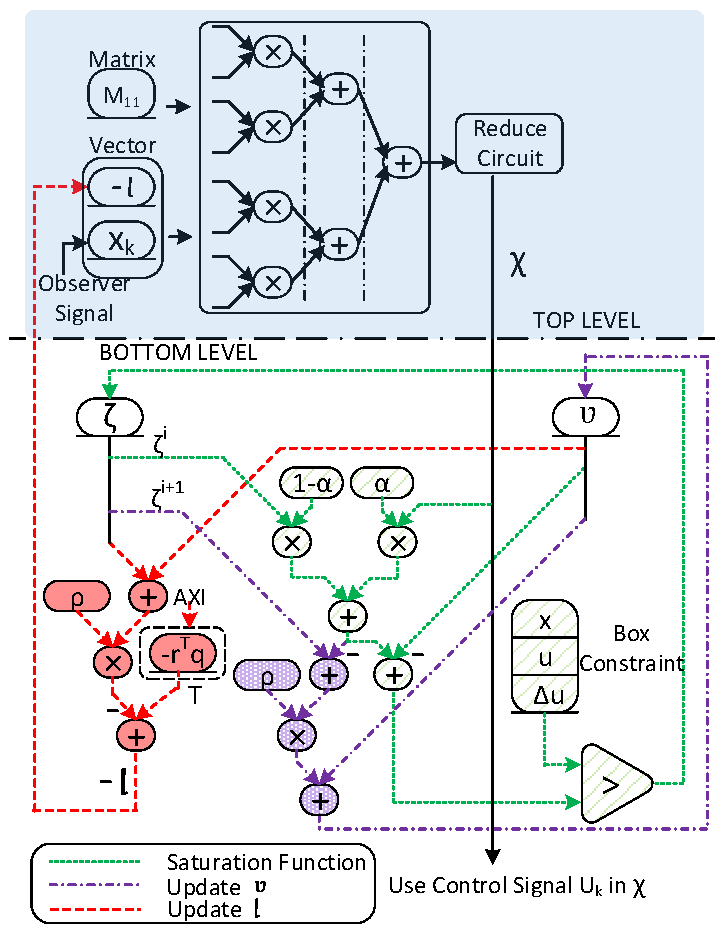
\includegraphics[scale=.45]{../ASAP_17/figure/architecture.pdf}
\DeclareGraphicsExtensions.
%\caption{Hardware Architecture for ADMM with Relaxation Parameter $\alpha$.\label{fig_arch}}
\end{figure}

\end{frame}
%------------------------------------------------
\begin{frame}
\frametitle{Hardware Architecture}
\framesubtitle{Processing Flow}
\begin{columns}[c] % The "c" option specifies centered vertical alignment while the "t" option is used for top vertical alignment
\column{.45\textwidth} % Left column and width
%\tikz[baseline,remember picture]{\node[anchor=base,marked on=<2->] (t1){
\uncover<1->{\alert<1>{\begin{block}{Step 1}
Solve KKT
\end{block}}}
\uncover<2->{\alert<2>{\begin{block}{Step 2}
Saturation Function
\end{block}}}
\uncover<3->{\alert<3>{\begin{block}{Step 3}
Update $\upsilon$
\end{block}}}
\uncover<4->{\alert<4>{\begin{block}{Step 4}
Update $l$
\end{block}}}


\column{.40\textwidth} % Right column and width
\begin{figure}[t]
\begin{tikzpicture}
\node[anchor=south west,inner sep=0] at (0,0) {
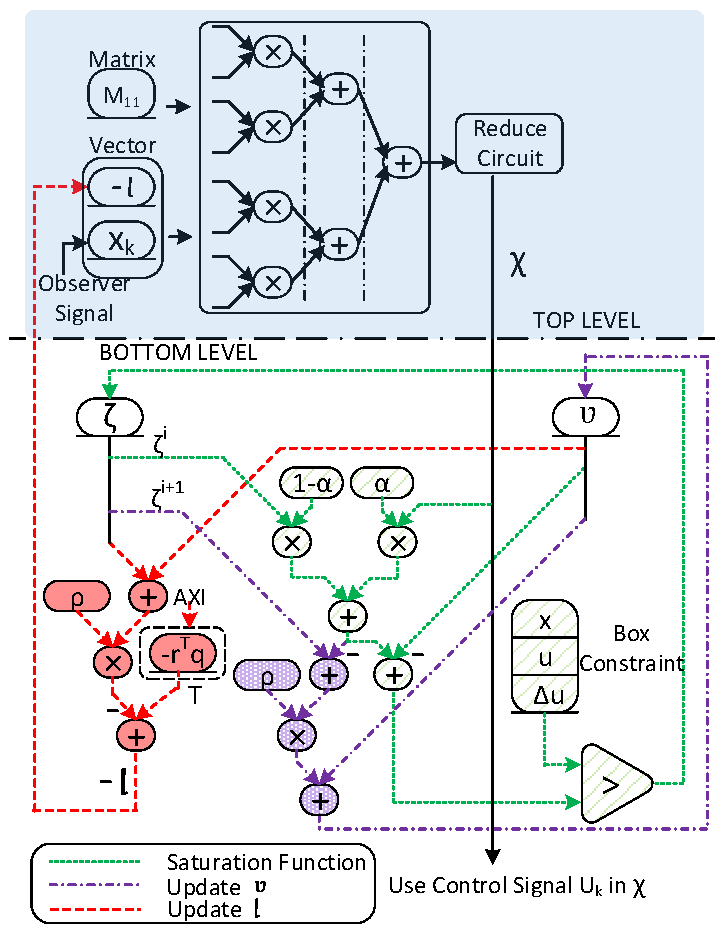
\includegraphics[scale=.40]{../ASAP_17/figure/architecture.pdf}
};
	\draw<1>[red,ultra thick,rounded corners,fill=orange,fill opacity=0.2] (0.1,3.9) rectangle (4.9,6.3);
	\draw<2>[red,ultra thick,rounded corners,fill=orange,fill opacity=0.2] (1,3)--(2,2)--(2.5,2)--(2.5,0.7)--(4.9,0.7)--(4.9,3.9)--(0.4,3.9)--(0.4,3.3)--(1,3);
	\draw<3>[red,ultra thick,rounded corners,fill=orange,fill opacity=0.2] (1.5,0.7) rectangle (2.5,2.0);
	\draw<4>[red,ultra thick,rounded corners,fill=orange,fill opacity=0.2] (0.2,1.0) rectangle (1.6,2.8);
	
\end{tikzpicture}
\end{figure}
\end{columns}




\end{frame}





%------------------------------------------------
\begin{frame}
\frametitle{Hardware Architecture}
\framesubtitle{Reduce Circuit}
\begin{figure}[t]
\centering
\captionsetup{justification=centering}
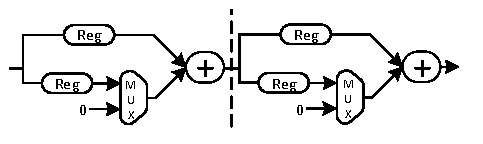
\includegraphics[scale=0.9]{../ASAP_17/figure/Reduce.pdf}
\DeclareGraphicsExtensions.
\caption{Reduce Circuit Architecture with Two Cascaded Adders\label{fig_red}}
\end{figure}
\end{frame}
%------------------------------------------------
\begin{frame}
\frametitle{Hardware Architecture}
\framesubtitle{Reduce Circuit}
\begin{figure}[t!]
\begin{tikzpicture}
\node[anchor=south west,inner sep=0] at (0,0) {
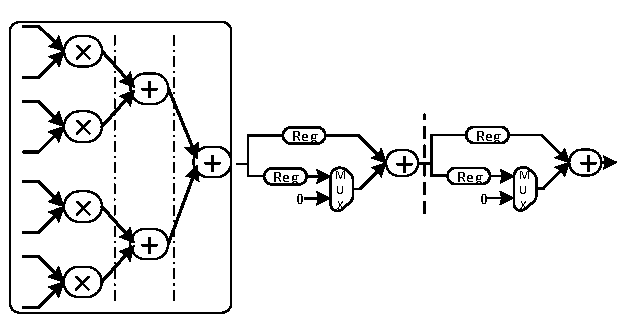
\includegraphics[scale=.45]{../pic/r_m.pdf}};
\end{tikzpicture}
\end{figure}

\setcounter{MaxMatrixCols}{20}
\begin{equation*}
\arraycolsep=3pt
\scalemath{0.8}{
G=
}
\scalemath{0.6}{
\begin{bmatrix}
   I & \dots & \dots & \dots  & \dots &\dots & \dots & \dots &\dots &\dots & \dots & \dots&\dots &\dots & \dots & \dots\\
   A & -I & \dots & \dots  & \dots & \dots & B & \dots & \dots &\dots &\dots & \dots & \dots &\dots &\dots & \dots\\
	\dots & A & -I & \dots & \dots & \dots& \dots&B& \dots &\dots &\dots & \dots & \dots &\dots &\dots & \dots\\
	\dots & \dots  & \dots & \dots & \dots & \dots  & \dots &\dots &\dots & \dots & \dots &B & \dots &\dots &\dots & \dots\\
\vdots & \vdots & \vdots & \vdots & \vdots & \vdots  & \vdots & \vdots  & \vdots & \vdots & \vdots & \vdots  & \vdots & \vdots & \vdots & \vdots\\
\dots & \dots & \dots & \dots & A & -I & \dots & \dots & \dots & \dots & \dots & B & \dots &\dots &\dots & \dots\\
\dots & \dots & \dots & \dots & \dots & \dots & I & -I & \dots & \dots & \dots & \dots & I & \dots  & \dots  & \dots\\ 
\dots & \dots & \dots & \dots & \dots & \dots &\dots  & I & -I & \dots & \dots & \dots & \dots & I  & \dots & \dots\\
\vdots & \vdots & \vdots & \vdots & \vdots & \vdots  & \vdots & \vdots  & \vdots & \vdots & \vdots & \vdots  & \vdots & \vdots & \vdots & \vdots\\
\dots & \dots & \dots & \dots & \dots & \dots &\dots  &\dots &\dots &\dots & I & -I &\dots & \dots & \dots & I
\end{bmatrix}}
\label{eq:g}
\end{equation*}

\end{frame}
%------------------------------------------------



\subsection{Trajectory Setting During Runtime}
%------------------------------------------------
\begin{frame}
\frametitle{Hardware Architecture}
\framesubtitle{Runtime Trajectory Planning}
\begin{figure}[t]
\centering
\captionsetup{justification=centering}
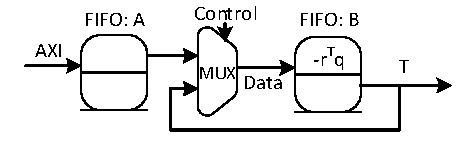
\includegraphics[scale=.75]{../ASAP_17/figure/trajectoryProfile.pdf}
\DeclareGraphicsExtensions.
\caption{Runtime Trajectory Planning\label{fig_traj}}
\end{figure}
\end{frame}


%------------------------------------------------

\subsection{Latency Analysis}
%------------------------------------------------
\begin{frame}
\frametitle{Latency of Each Pipeline Stages}
\begin{columns}[c] % The "c" option specifies centered vertical alignment while the "t" option is used for top vertical alignment
\column{.450\textwidth} % Left column and width
\begin{figure}[t!]
\begin{tikzpicture}
\node[anchor=south west,inner sep=0] at (0,2.5) {
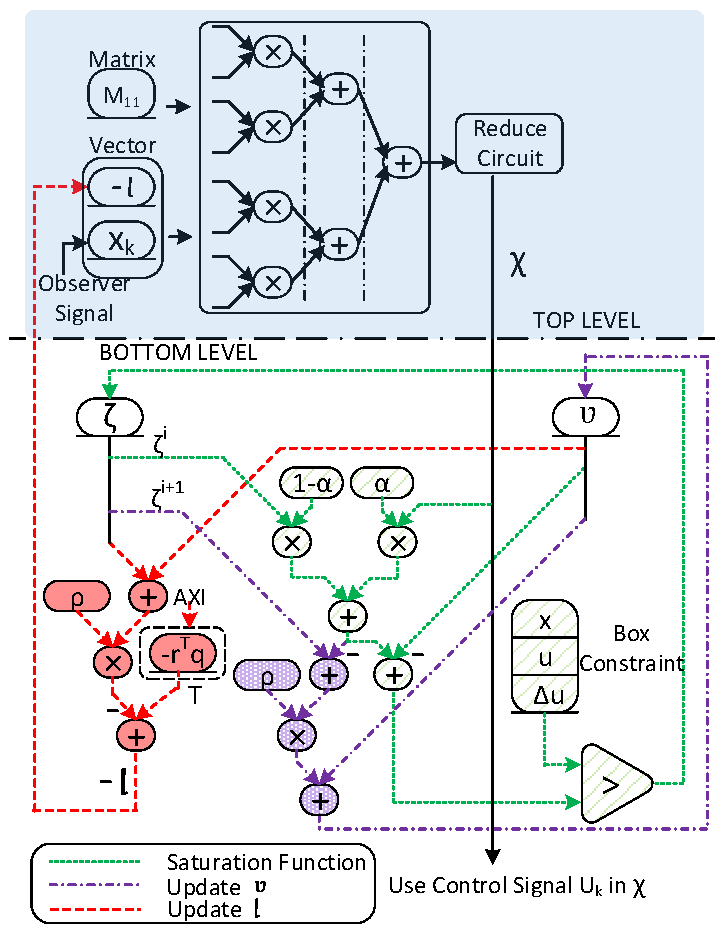
\includegraphics[scale=.35]{../ASAP_17/figure/architecture.pdf}};

\draw<1>[red,ultra thick,rounded corners,fill=orange,fill opacity=0.2] (0.6,6.2) rectangle (1.5,8.0);
\draw<2>[red,ultra thick,rounded corners,fill=orange,fill opacity=0.2] (1.2,6.1) rectangle (3.5,8.0);
\draw<3>[red,ultra thick,rounded corners,fill=orange,fill opacity=0.2] (0.1,2.8) rectangle (4.3,6.0);
\draw<4>[red,ultra thick,rounded corners,fill=orange,fill opacity=0.2] (0.1,2.8) rectangle (4.3,8.0);


\end{tikzpicture}
\end{figure}
\column{.50\textwidth} % Right column and width

\footnotesize{

The number of clock cycles to merge all the matrix and vector data into the MVM pipeline is:
\begin{equation*}
\label{eq:md}
\tikz[baseline,remember picture]{\node[anchor=base,marked on=<1>]{$L_{read\_ M_{11}}=N_{ROW}*(N_R+1)$};} 
\end{equation*}


\begin{equation*}
\tikz[baseline,remember picture]{\node[anchor=base,marked on=<2>] {$Binary Tree (L_{bt})=L_M+D_pL_A+N_R(L_A+2)$};} 
\end{equation*}

\begin{equation*}
\tikz[baseline,remember picture]{\node[anchor=base,marked on=<3>] {$ Bottom Level (L_{bl})=6L_A+3L_M+L_C $};}  
\end{equation*}

Total Latency:
\begin{equation*}
\label{eq:tl}
\tikz[baseline,remember picture]{\node[anchor=base,marked on=<4>] {$ L_{ADMM}=L_{bt}+L_{bl}+L_{read\_ M_{11}}$};}  
\end{equation*}

}

\end{columns}

\end{frame}
%------------------------------------------------

\section{Evaluation}
%------------------------------------------------
\begin{frame}
\frametitle{Mass-spring System (Testbench)}
\begin{figure}[t]
\centering
\captionsetup{justification=centering}
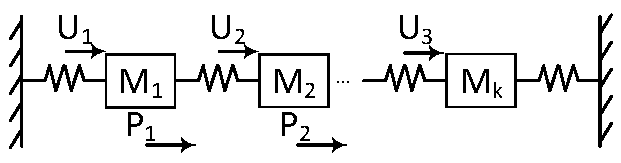
\includegraphics[scale=.48]{../ASAP_17/figure/massspring.pdf}
\DeclareGraphicsExtensions.
\caption{Mass-spring System\label{fig_ms}}
\end{figure}
\hrule
\begin{itemize}
	\item Objective: moving masses to desired positions by applying a force to each mass. 
	\item State Variable: position ($P$) and speed ($\dot P$) of each mass\footnote{$P$ is the position relative to the initial position}
	\item Constraints: 
\[
  \begin{cases*}
    -0.5m\leq P\leq 0.5m\\
    -0.5N\leq u\leq 0.5N\\
    -0.1N/s \leq \Delta u\leq 0.1N/s
  \end{cases*}\]
\end{itemize}
\end{frame}
%------------------------------------------------
\subsection{Plant on Chip}
\begin{frame}
\frametitle{Plant on Chip}
A hardware component that emulates the physical behavior of a linear system.
\begin{figure}
\begin{tikzpicture}
\node[anchor=south west,inner sep=0] at (-8,0.3) {
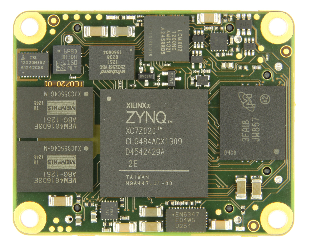
\includegraphics[scale=.35]{../pic/zynq.png}};

\node[anchor=south west,inner sep=0] at (-4.25,1.3) {

\includegraphics[scale=.10]{../pic/arrow.png}};

\draw<1>[red,ultra thick,rounded corners,fill=orange,fill opacity=0.2,xshift=-10.0, yshift=55] (-1.6,-0.8) rectangle (1.6,0.4);

\node<1>[color=black,xshift=-10.0, yshift=55] at (0,0) {
$x_{k+1}=A x_k + B u_k$ 
};
\node<1>[color=black,xshift=-10.0, yshift=55] at (0,-0.4) {
$y_{k}=C x_k + D u_k $ 
};

\draw<1>[red,ultra thick,rounded corners,xshift=10.5, yshift=55,->] (-3,-2)--(-3,0)--(-2.5,0);

\draw<1>[red,ultra thick,rounded corners,xshift=10.5, yshift=55,->] (1,0)--(1.5,0)--(1.5,-2);

\node<1>[color=black,xshift=-20.0, yshift=55] at (-2,-2.5) { Input: $u_k$};

\node<1>[color=black,xshift=-20.0, yshift=55] at (2.5,-2.5) { Sensor: $y_k$};

\end{tikzpicture}
\end{figure}

\end{frame}
%------------------------------------------------



\begin{frame}
\frametitle{Emulation using Plant on Chip}
\framesubtitle{Mass Position}
\begin{figure}[t]
\centering
\captionsetup{justification=centering}
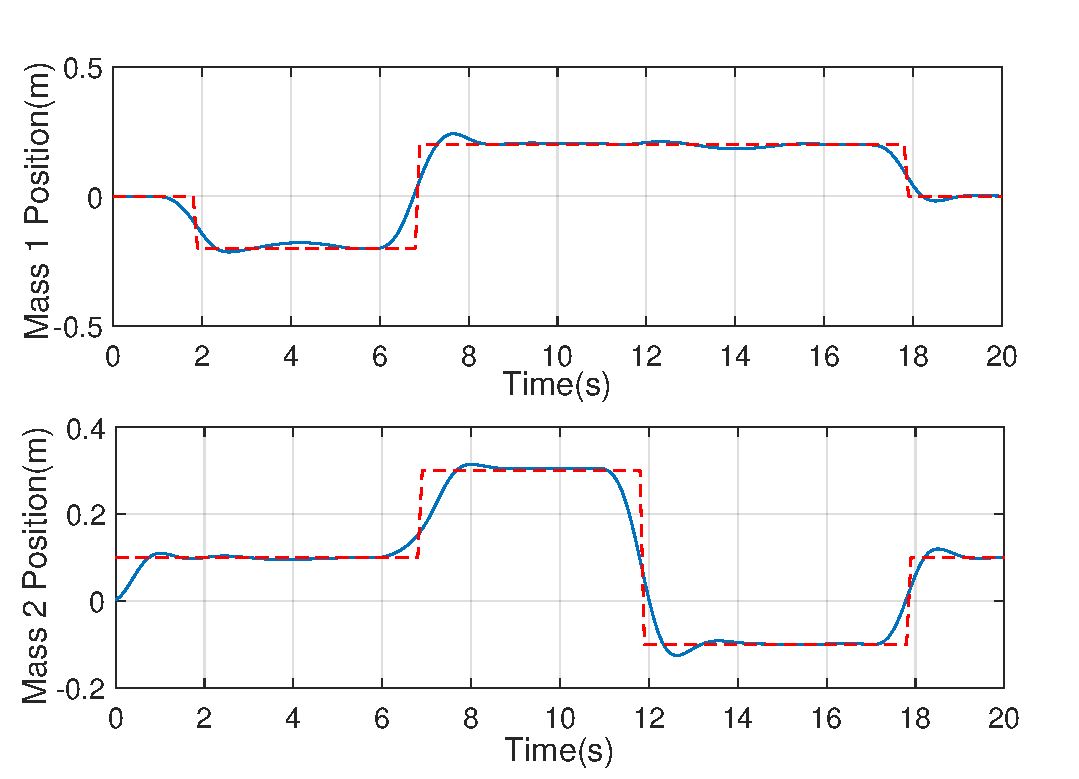
\includegraphics[scale=.45]{../ASAP_17/figure/MP.pdf}
\DeclareGraphicsExtensions.
\caption{Mass Position Change with respect to Planned Trajectory. Red dashed line is the planned trajectory, and the blue line is the actual trajectory.\label{fig_mp}}
\end{figure}
\end{frame}
%------------------------------------------------
\begin{frame}
\frametitle{Emulation using Plant on Chip}
\framesubtitle{Constraints on Force and its Rate of Change}
\begin{figure}[t]
\centering
\captionsetup{justification=centering}
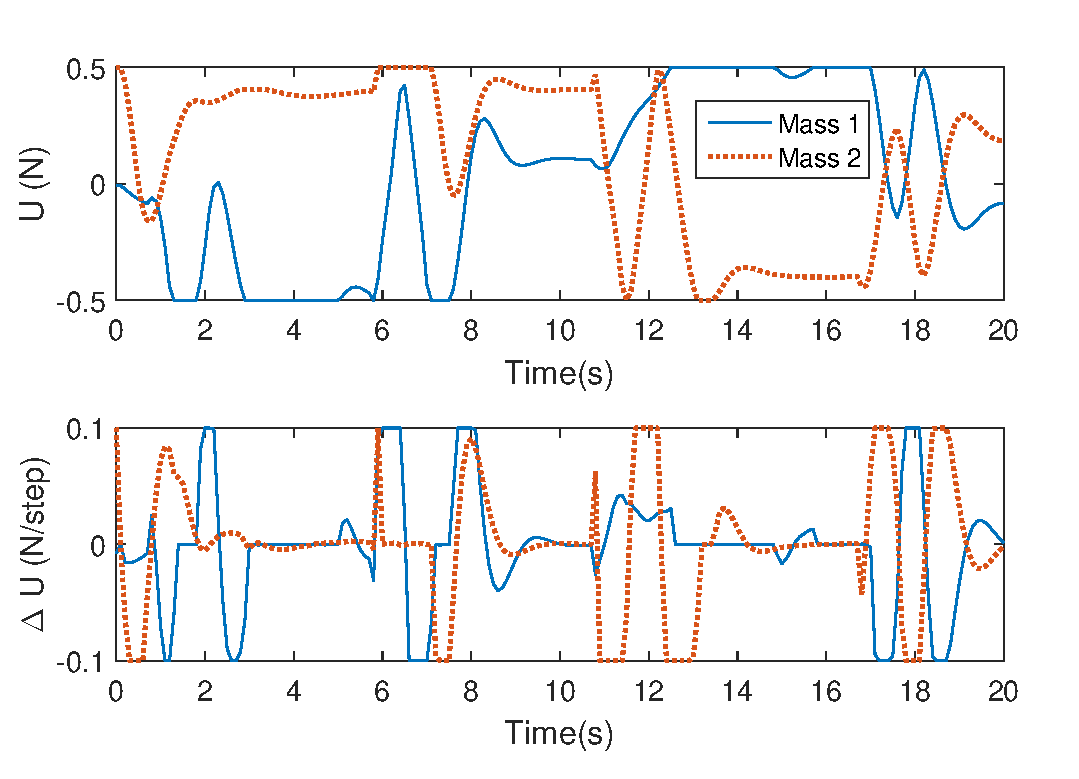
\includegraphics[scale=.45]{../ASAP_17/figure/MU.pdf}
\DeclareGraphicsExtensions.
\caption{Control Signal $U$ and $\Delta U$. Blue line is the input force and the force rate of change for $M_1$, red dashed line is for $M_2$.\label{fig_mu}}
\end{figure}
\end{frame}
%------------------------------------------------

%------------------------------------------------
\subsection{SW/HW Co-design}
\begin{frame}
\frametitle{SW/HW Co-design}
\begin{figure}[t]
\centering
\captionsetup{justification=centering}
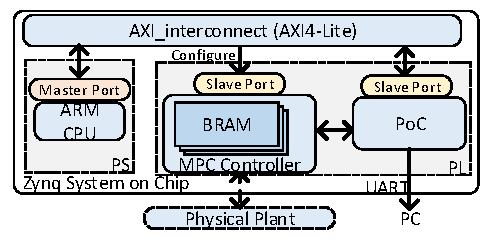
\includegraphics[scale=.84]{../ASAP_17/figure/copro.pdf}
\DeclareGraphicsExtensions.
\caption{Top Level System Overview\label{fig_copro}}
\end{figure}

\end{frame}
%------------------------------------------------
\begin{frame}
\frametitle{Deploy Steps}
\begin{columns}[c] % The "c" option specifies centered vertical alignment while the "t" option is used for top vertical alignment
\column{.43\textwidth} % Left column and width

\uncover<1->{\alert<1>{\begin{block}{Step 1}
\small{According to system requirements, generate the bitstream in Vivado, and $M_{11}$ matrix in Matlab.}
\end{block}}}
\uncover<2->{\alert<2>{\begin{block}{Step 2}
\small{Store $M_{11}$ to BRAM via AXI bus using ARM software.}
\end{block}}}
\uncover<3->{\alert<3>{\begin{block}{Step 3}
\small{ARM software configures trajectory and box constraints.}
\end{block}}}


\column{.49\textwidth} % Right column and width
\begin{figure}[t!]
\begin{tikzpicture}
\node[anchor=south west,inner sep=0] at (0,0) {
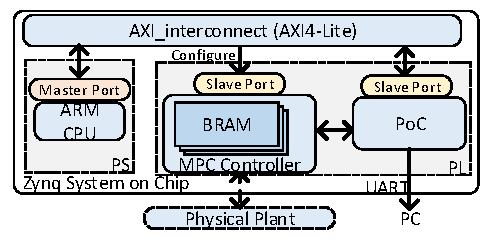
\includegraphics[scale=.74]{../ASAP_17/figure/copro.pdf}};


\node<1>[draw,color=red] at (1,3.2) {$M_{11}$};
\node<1>[draw,color=red,fill=orange,fill opacity=0.7] at (3,3.2) {Bitfile};
\draw<1>[red,ultra thick,rounded corners,->] (3.6,3.2)--(4.1,3.2) -- (4.1,2);
\node<2>[draw,color=red,fill=orange,fill opacity=0.7] at (1,1.2) {$M_{11}$};
\draw<2>[red,ultra thick,rounded corners,->] (1,1.4)--(1,2.7) -- (2.9,2.7)--(2.9,1.7);
\node<3>[draw,color=red,fill=orange,fill opacity=0.7] at (5,-0.1) {Trajectory};
\draw<3>[red,ultra thick,rounded corners,->] (5,0)--(5,0.7)--(0.9,0.7) -- (0.9,2.7)--(2.9,2.7)--(2.9,1.7);

\node<4>[draw,color=red,fill=green,fill opacity=0.7] at (4.4,-0.1) {Start};
\node<4>[draw,color=red,fill=orange,fill opacity=0.7] at (5.4,-0.1) {Data};
\draw<4>[red,ultra thick,rounded corners,->] (4.4,0)--(4.4,0.7)--(0.9,0.7) -- (0.9,2.7)--(5.2,2.7)--(5.2,1.7);
\draw<4>[red,ultra thick,rounded corners,->] (5.4,1.2)--(5.4,0);
\draw<4>[red,ultra thick,rounded corners,->] (3,2.7)--(3,1.7);
\end{tikzpicture}
\end{figure}

\uncover<4->{\alert<4>{\begin{block}{Step 4}
\small{Send start signal to the PoC, and collect data through UART to external computer and plot graph.}
\end{block}}}

\end{columns}
\end{frame}

%------------------------------------------------
\begin{frame}
\frametitle{Computation Speed Versus Hardware Resources}
\begin{figure}[t]
\centering
\captionsetup{justification=centering}
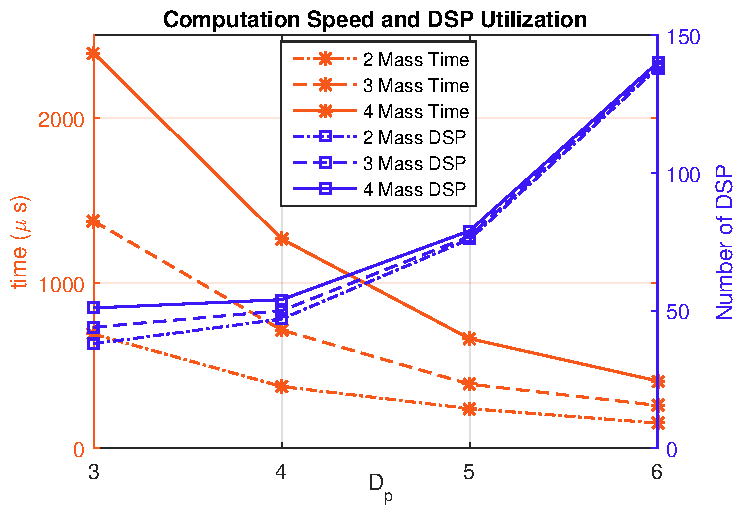
\includegraphics[scale=.65]{../ASAP_17/figure/dsp.pdf}
\DeclareGraphicsExtensions.
\caption{Computation time of 40 converge iteration loops and DSP usage for different system configurations from simulation. Computation time is marked by $\ast$, number of DSPs is marked by $\Box$. Hardware speed is 100MHz.\label{fig_ct}}
\end{figure}

\end{frame}
%------------------------------------------------
\begin{frame}
\frametitle{Potential Computation Parallism}

\begin{figure}[t!]
\begin{tikzpicture}
\node[anchor=south west,inner sep=0] at (-1.5,1) {
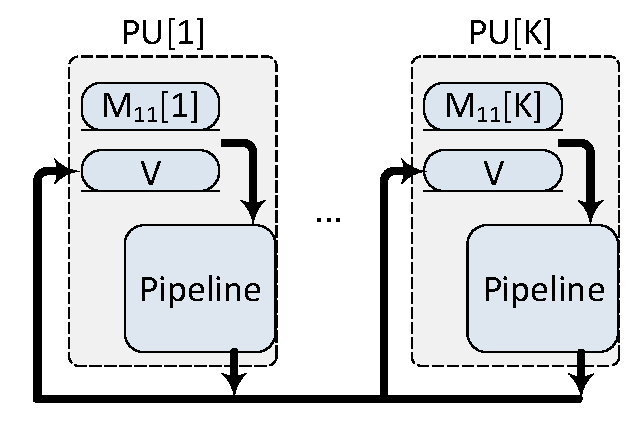
\includegraphics[scale=.55]{../ASAP_17/figure/highParallel.pdf}};
\node[anchor=south west,inner sep=0] at (6.5,1.8) {
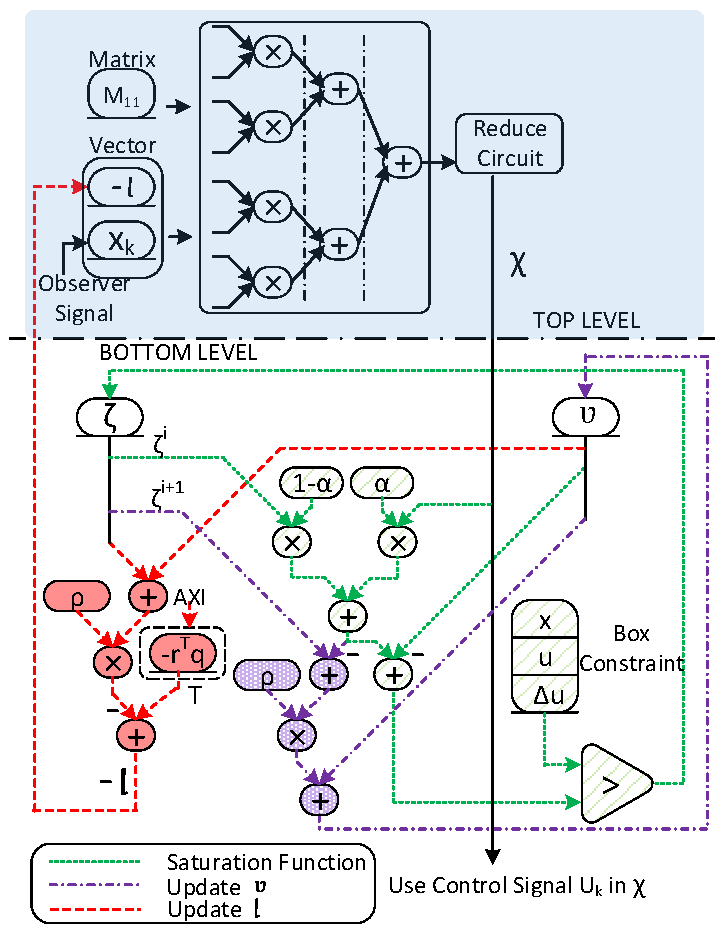
\includegraphics[scale=.15]{../ASAP_17/figure/architecture.pdf}};
\draw[red,ultra thick,rounded corners,->] (4,1.3)--(6.5,1.7);
\draw[red,ultra thick,rounded corners,->] (4,4.5)--(6.5,4.1);

\end{tikzpicture}
\end{figure}


%\begin{figure}[!ht]
%\centering
%\captionsetup{justification=centering}
%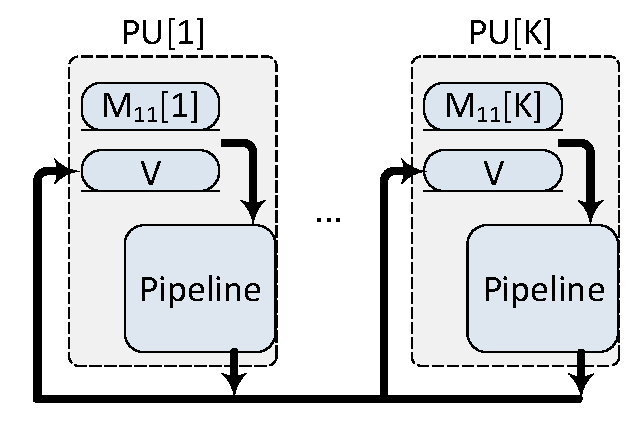
\includegraphics[scale=.55]{../ASAP_17/figure/highParallel.pdf}
%\DeclareGraphicsExtensions.
%\caption{Highly paralleled ADMM Hardware Solution\label{fig_hp}}
%\end{figure}



$L_{read\_ M_{11}}$ is inverse proportional to parallelism $K$.
\begin{equation}
\label{eq:klemr}
L_{read\_ M_{11}}=\frac{N_{ROW}}{K}*(N_R+1)
\end{equation}

\end{frame}



%------------------------------------------------
\begin{frame}
\frametitle{Resource Utilization}
\begin{table}[!ht]
\centering
\captionsetup{justification=centering}
\caption{Zynq-7020 Hardware Resource Usage}\label{tab_hrs}
\resizebox{3in}{!}{%
\begin{tabular}{ >{\centering\arraybackslash} m{1cm} |>{\centering\arraybackslash} m{1.4cm}|>{\centering\arraybackslash} m{1.4cm}|>{\centering\arraybackslash} m{1.4cm}|>{\centering\arraybackslash} m{1cm}|>{\centering\arraybackslash} m{1.4cm} }

\hline
\multicolumn{1}{c|}{MVM}&\multicolumn{1}{c|}{Flip-Flops}&\multicolumn{1}{c|}{LUTs}&\multicolumn{1}{c|}{18Kb BRAM}&\multicolumn{1}{c|}{DSP48E}&\multicolumn{1}{c}{Maximum}\\

Size $D_p$ &(106400 total)&(53200 total)&(280 total)&(220 total)&Frequency \\ 
 
\hline

3&18147&12746&55&38&151.149MHz\\
\hline 
4& 21058 & 15103&87&47&144.885MHz\\
\hline 
5& 32425 & 23391 &151&76&143.699MHz\\
\hline 
6& 57167 & 41273&279&138&133.298MHz\\
\hline

\end{tabular}}
\end{table}
\end {frame}

%------------------------------------------------
\begin{frame}
\frametitle{Timing Summary}
 \begin{table}[!ht]
\small
\centering
\captionsetup{justification=centering}
\caption{Hardware Computation Time per Iteration between Related Work.\label{tab_cmp}}
\resizebox{\columnwidth}{!}{%
\begin{tabular}{|*{9}{c|}}\hline

&\makebox[2.2em]{Method}&\makebox[4em]{Data Format}&\makebox[4em]{Chip Series}&\makebox[2.5em]{$f_{clk}$}&\makebox[4em]{\#Multipliers}&\makebox[2.5em]{Iteration}&\makebox[3em]{\#Opt Var}&\makebox[6em]{Running Time}\\
\hline
\hline

\multirow{5}{*}{This Paper} &\multirow{5}{*}{ADMM}&\multirow{5}{*}{floating-point}&\multirow{3}{*}{Zynq-7020}&\multirow{3}{*}{130MHz}&\multirow{2}{*}{72 ($D_p$=6, K=1)}&\multirow{5}{*}{40}&\multirow{1}{*}{204}&\multirow{1}{*}{314.2 $\mu s$}\\
\hhline{~~~~~~~--}
&&&\multirow{0}{*}{}&&&&350*&{717.2 $\mu s$}\\
\hhline{~~~~~-~--} 
&&&\multirow{1}{*}{}&&80 ($D_p$=5, K=2)&&\multirow{3}{*}{204}&{291.4 $\mu s$}\\
\hhline{~~~---~~-}
&&&\multirow{1}{*}ZU9EG&\multirow{2}{*}{340MHz}&264 ($D_p$=8, K=1)&&&{46.1 $\mu s$}\\
\hhline{~~~~~-~~-}
&&&\multirow{1}{*}(Zynq UltraScale+)&&792 ($D_p$=8, K=3)&&&{30.1 $\mu s$}\\ 
\hline
\hline

\multirow{2}{*}{HW\cite{jerez2014embedded}} &\multirow{2}{*}{ADMM}&\multirow{2}{*}{fixed-point}&Virtex-6 (LX75)&\multirow{2}{*}{400MHz}&\multirow{1}{*}{216 (K=1)}&\multirow{2}{*}{40}&\multirow{2}{*}{216}&\multirow{1}{*}{23.4$\mu s$}\\ 
\hhline{*4~|*1~|*4~}
%&&&LX75&& &&&\\
\hhline{*3~|-|~|-|*2~|-}
\multirow{1}{*}{} &\multirow{1}{*}{}&\multirow{1}{*}{}&Virtex-6 (SX475)&\multirow{0}{*}{}&\multirow{1}{*}{1512 (K=7)}&\multirow{1}{*}{}&\multirow{1}{*}{}&\multirow{1}{*}{4.90$\mu s$}\\ 
\hhline{*4~|*1~|*4~}
%&&&SX475&& &&&\\
\hline
\hline

\multirow{1}{*}{HW\cite{6927473}} &\multirow{1}{*}{IPM}&\multirow{1}{*}{floating-point}&Virtex-7 (XC7VX485T)&\multirow{1}{*}{200MHz}&\multirow{1}{*}{448}&\multirow{1}{*}{10}&\multirow{1}{*}{240}&\multirow{1}{*}{2,650 $\mu s$}\\ 
\hhline{*9~}
%&&&(XC7VX485T)&&&&&\\
\hline
\hline

\multirow{1}{*}{SW\cite{6422363}} &\multirow{1}{*}{ADMM}&\multirow{1}{*}{floating-point}& Quad-core Intel
Xeon&\multirow{1}{*}{3.4GHz}&\multirow{1}{*}{n/a}&\multirow{1}{*}{35.1}&\multirow{1}{*}{525}&\multirow{1}{*}{3,400 $\mu s$}\\ 
\hhline{*9~}

\hline
\end{tabular}
}
\end{table}



\end{frame}
%------------------------------------------------





\section{Conclusion}
\begin{frame}
\frametitle{Summary of Work}
The primary contribution of this work is a software/hardware (SW/HW) co-design that allows:
\begin{itemize}
\item configuring an MPC controller for a wide range of plants;
\item updating at run-time the desired trajectory to track;
\item the flexibility to trade off hardware resources for computing speed;
\item easing controller deployment by introducing an SW/HW co-design to decouple hardware details from control and embedded software engineers.
\end{itemize}

\end{frame}


%------------------------------------------------


%------------------------------------------------


%------------------------------------------------


%------------------------------------------------




%------------------------------------------------

\begin{frame}[fragile] % Need to use the fragile option when verbatim is used in the slide
\frametitle{Citation}
An example of the \verb|\cite| command to cite within the presentation:\\~

This statement requires citation \cite{p1}.
\end{frame}

%------------------------------------------------

\begin{frame}
\frametitle{References}
\footnotesize{
\begin{thebibliography}{99} % Beamer does not support BibTeX so references must be inserted manually as below
\bibitem[Smith, 2012]{p1} John Smith (2012)
\newblock Title of the publication
\newblock \emph{Journal Name} 12(3), 45 -- 678.
\end{thebibliography}
}
\end{frame}

%------------------------------------------------

\begin{frame}
\Huge{\centerline{The End}}
\end{frame}

%----------------------------------------------------------------------------------------

\end{document} 